\section{Performance}
\label{sec:perf}

The MMTP performs admirably.

\subsection{Low-level performance}
\label{sec:perf-simple}

\subsection{Roads}

\subsection{Resolution}
\label{sec:perf-res}

\subsubsection{Spatial and angular resolution}

\begin{figure}[!htpb]
  \begin{center}
    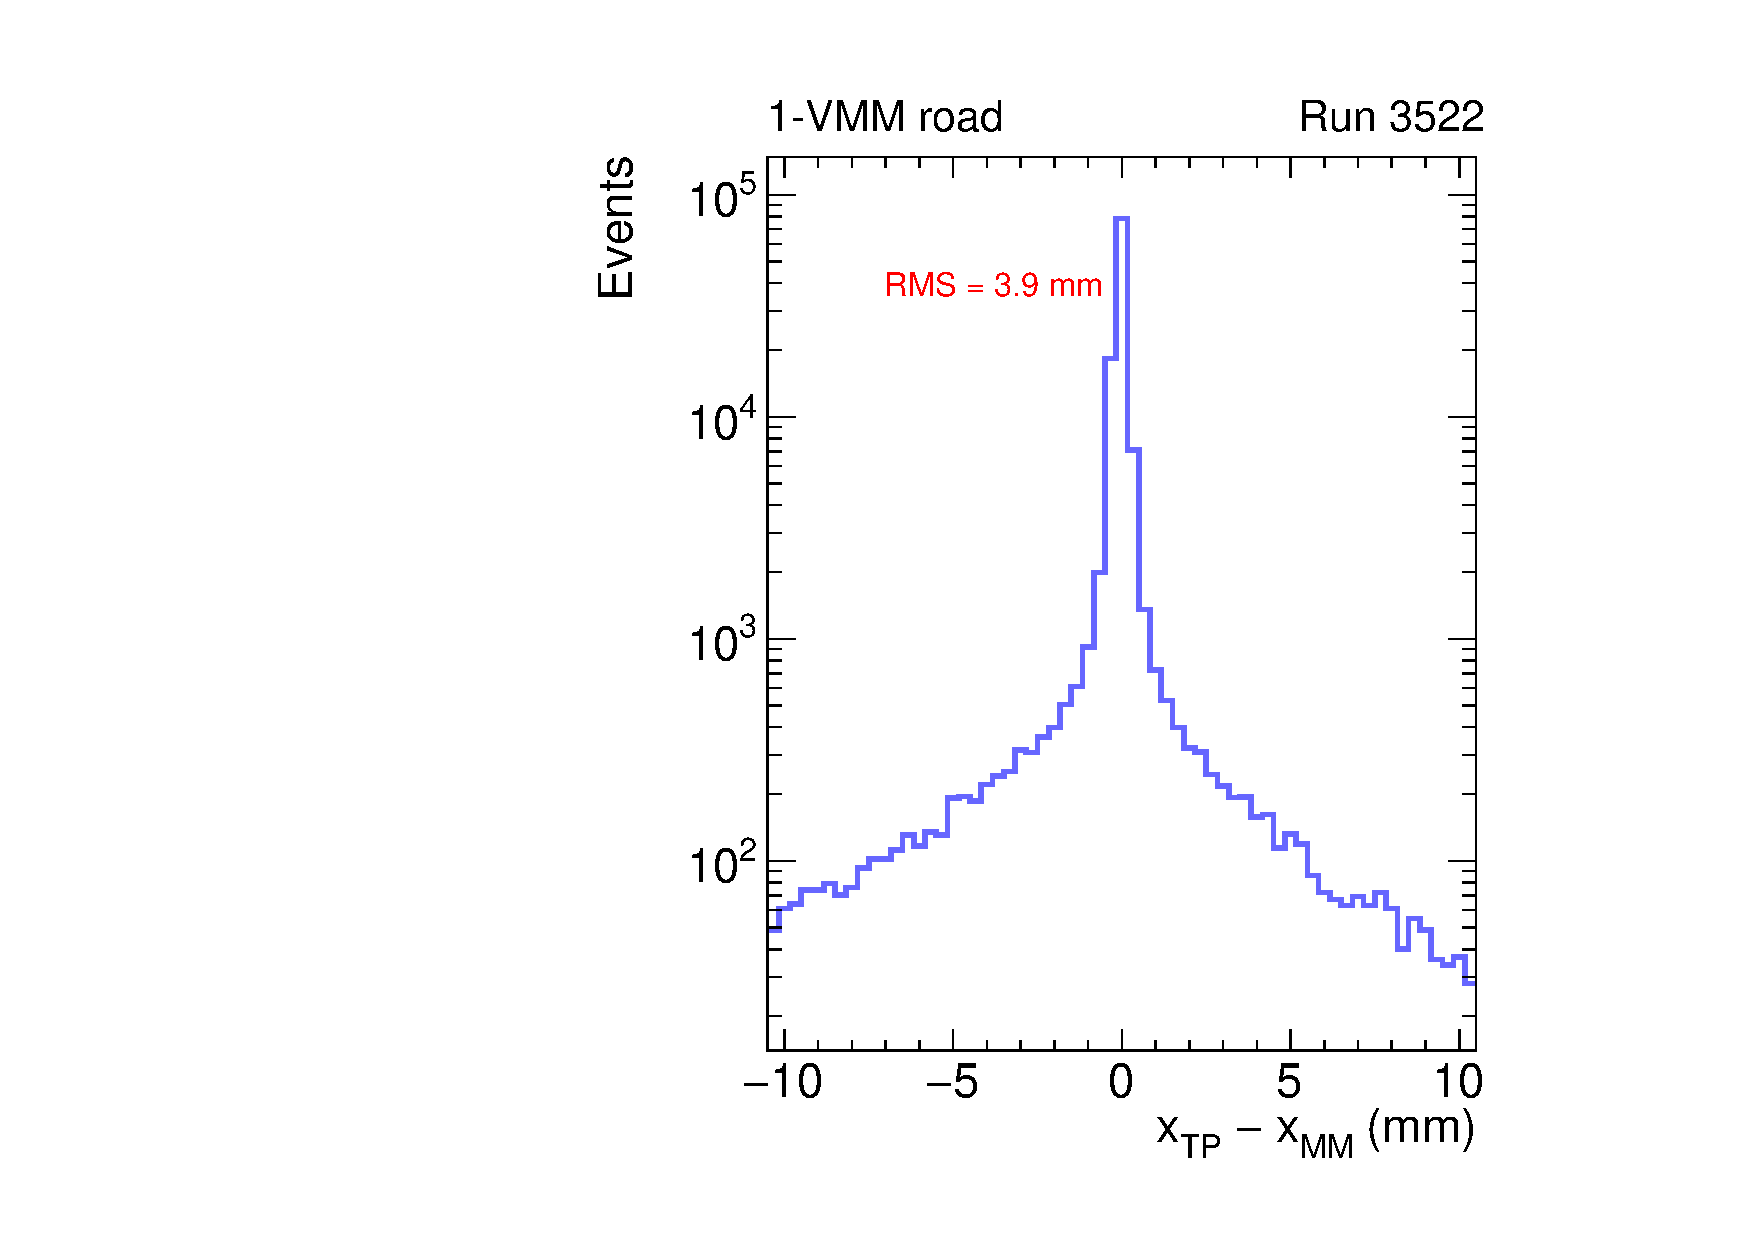
\includegraphics[width=0.4\textwidth]{figures/gbtanalysis3522/TP_xres_full.pdf}
    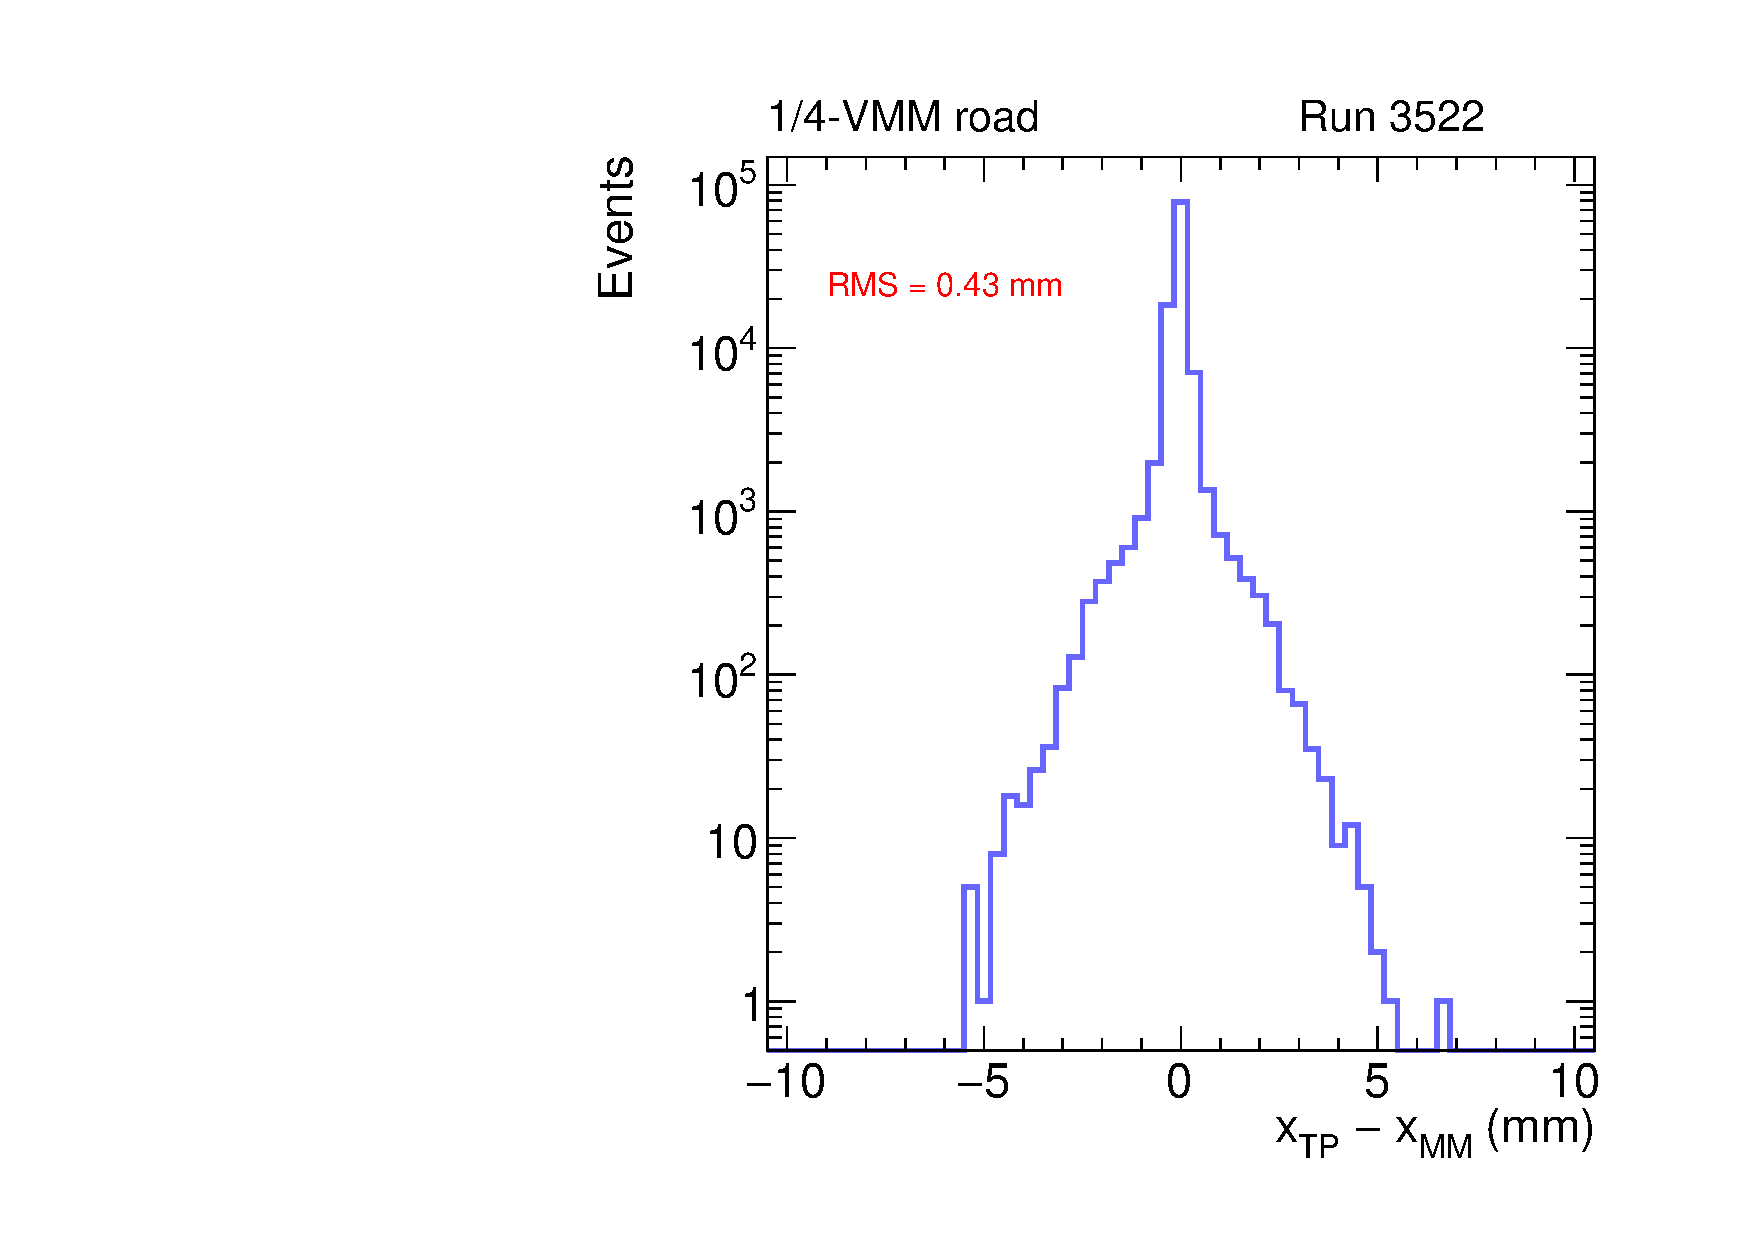
\includegraphics[width=0.4\textwidth]{figures/gbtanalysis3522/TP_xres.pdf}
  \end{center}
  \vspace{-10pt}
  \caption{The $x$ resolution of the MM TP relative to the full readout, using 1-VMM online roads (left) and 1/4-VMM offline roads (right). The tails of the resolution are greatly suppressed with smaller roads.}
  \label{fig:xres}
\end{figure}

\begin{figure}[!htpb]
  \begin{center}
    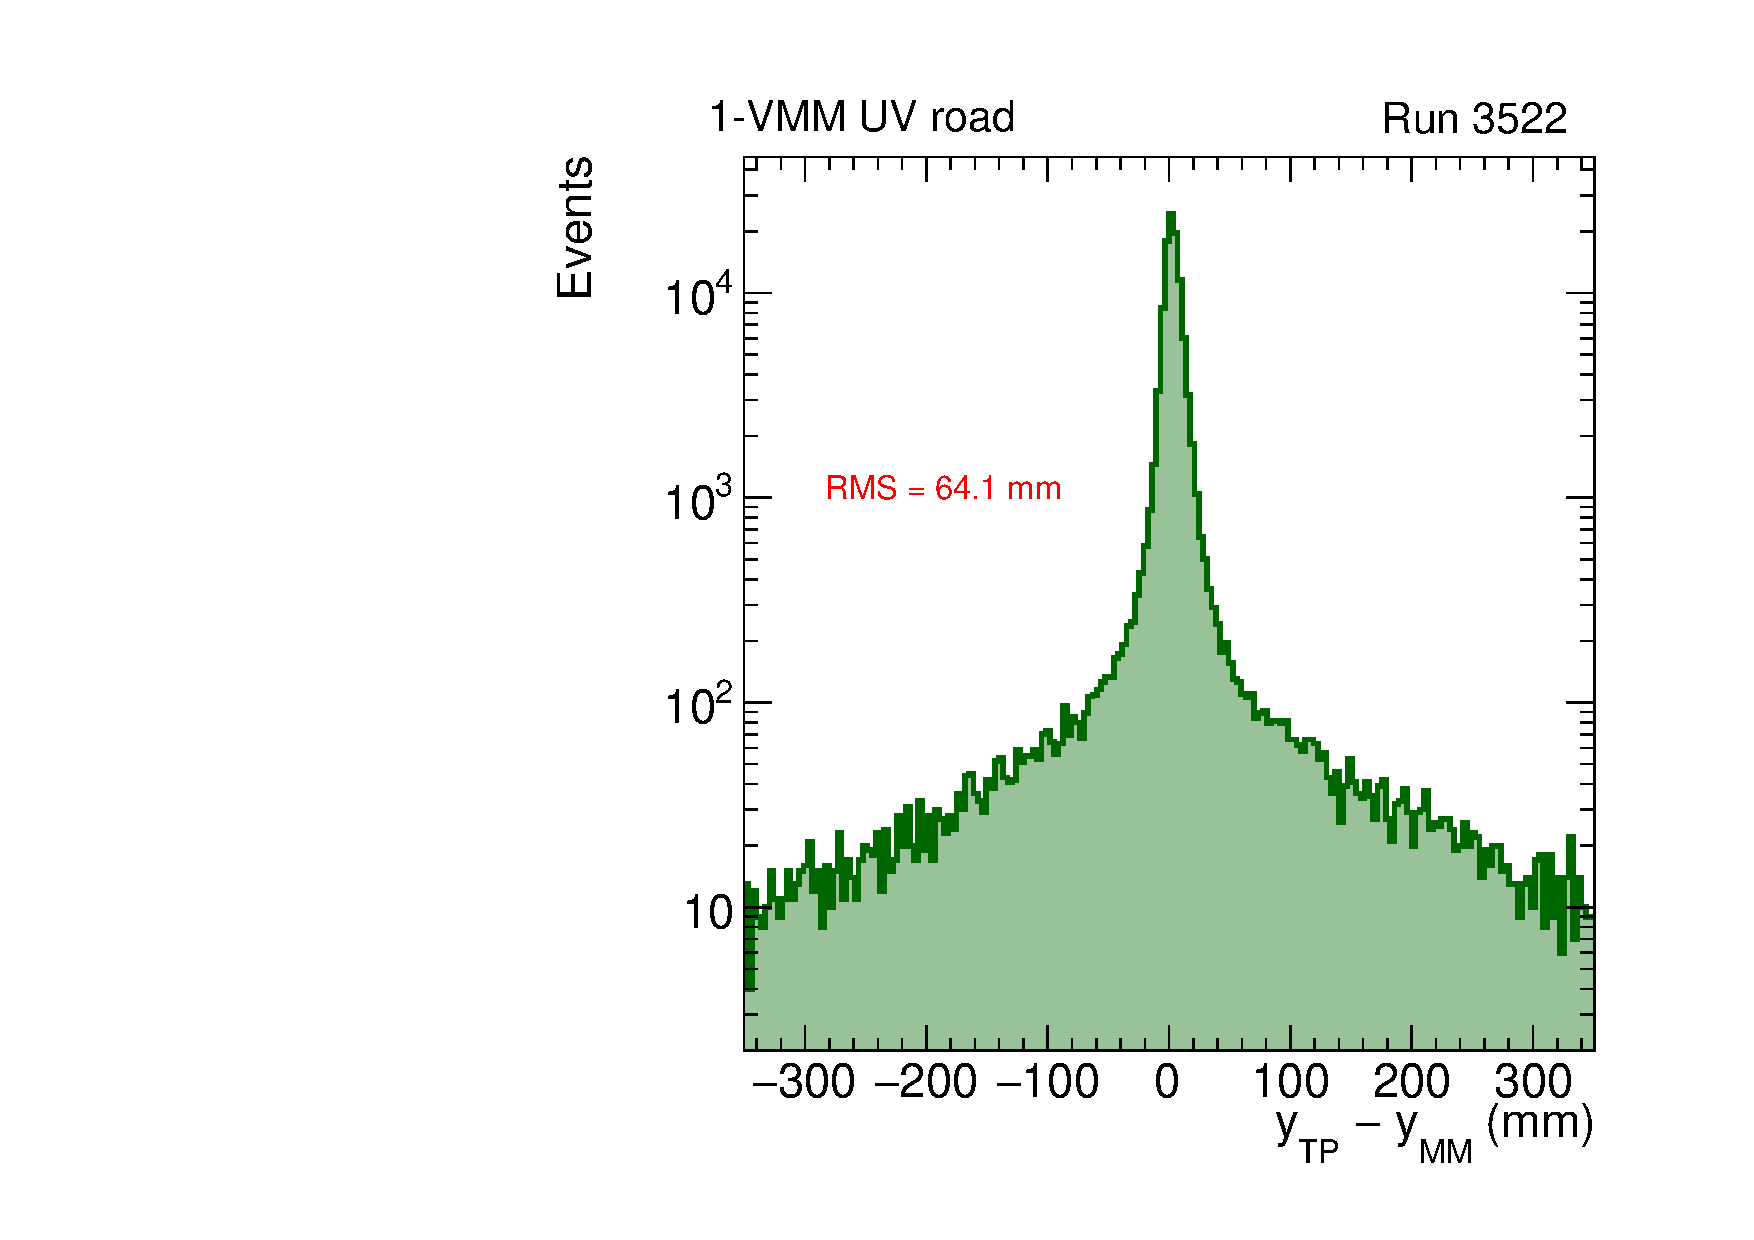
\includegraphics[width=0.4\textwidth]{figures/gbtanalysis3522/TP_yres_1road.pdf}
    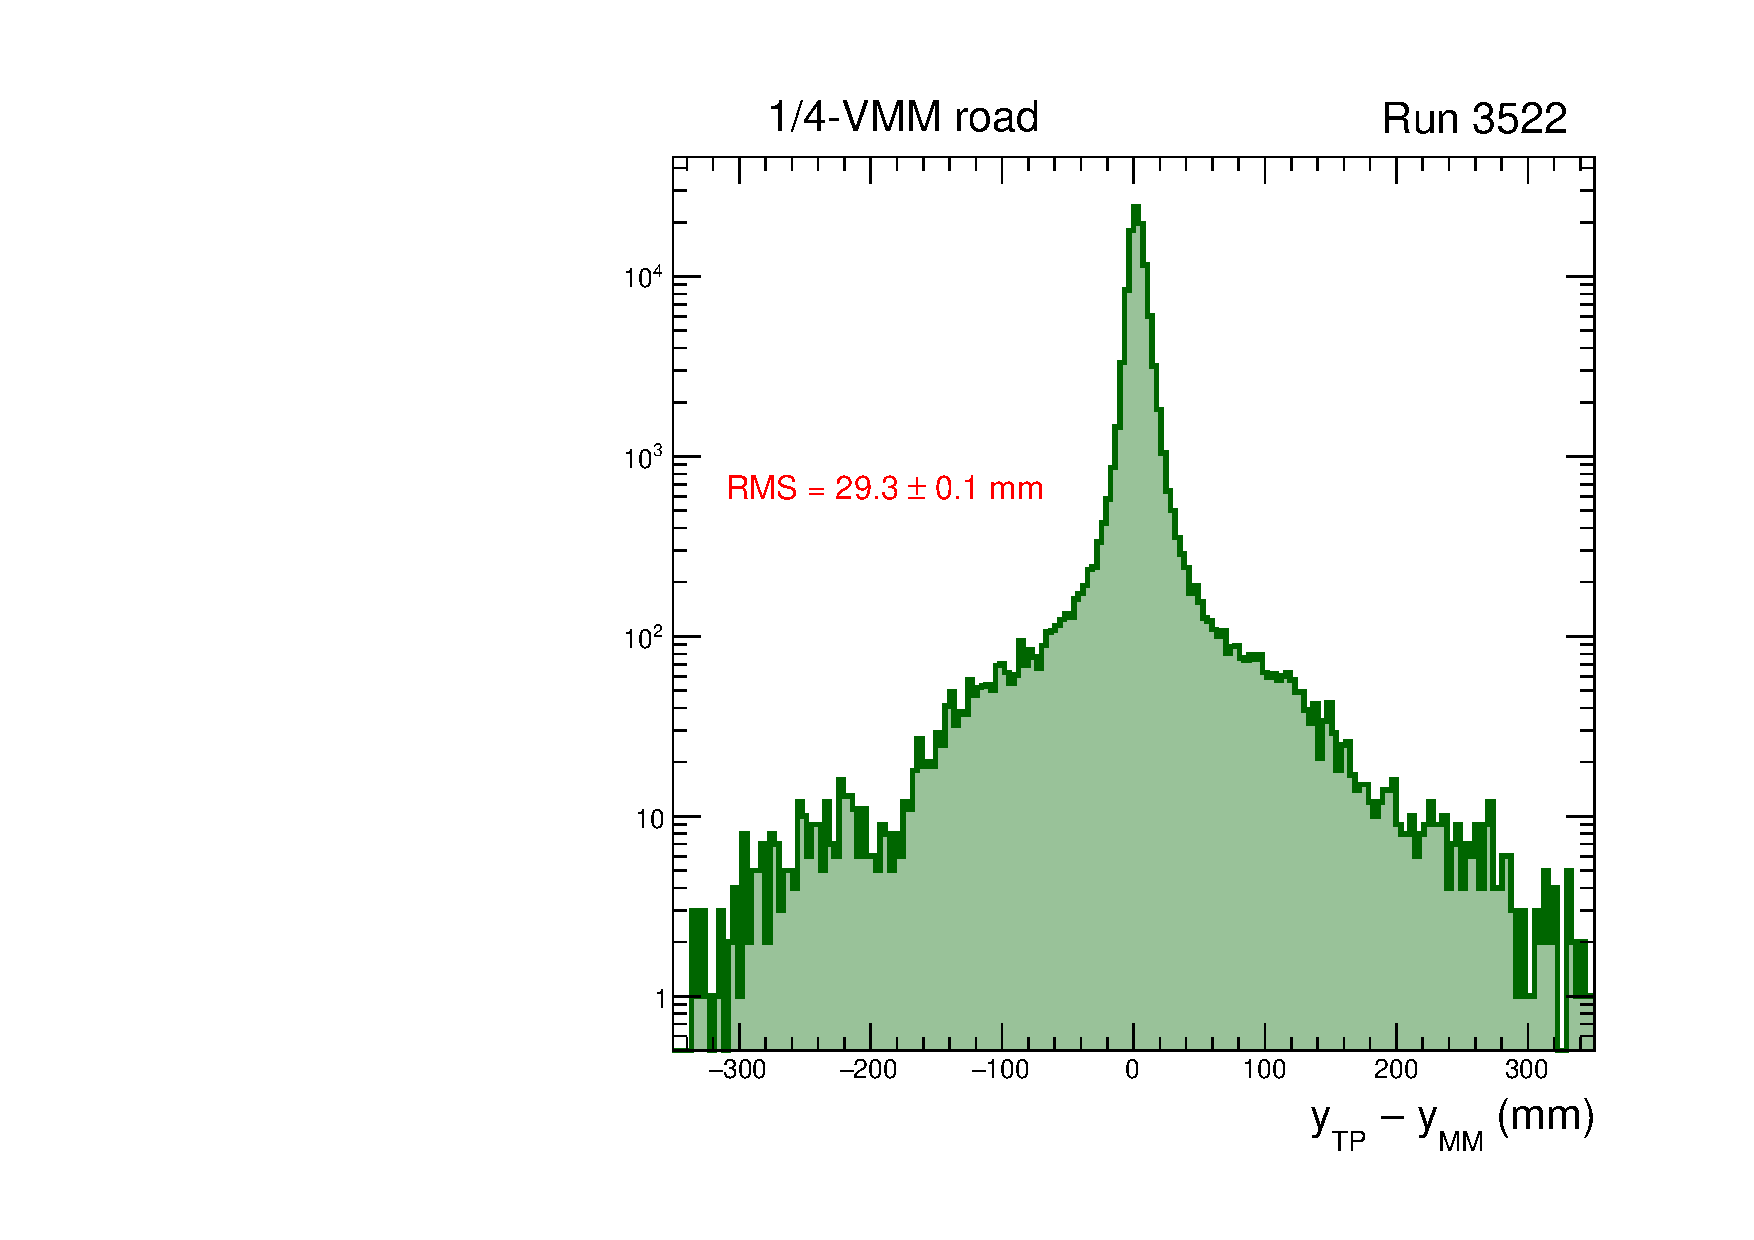
\includegraphics[width=0.4\textwidth]{figures/gbtanalysis3522/TP_yres_smallroad.pdf}
  \end{center}
  \vspace{-10pt}
  \caption{The $y$ resolution of the MM TP relative to the full readout, using 1-VMM online roads (left) and 1/4-VMM offline roads (right). The tails of the resolution are greatly suppressed with smaller roads.}
  \label{fig:yres}
\end{figure}

\begin{figure}[!htpb]
  \begin{center}
    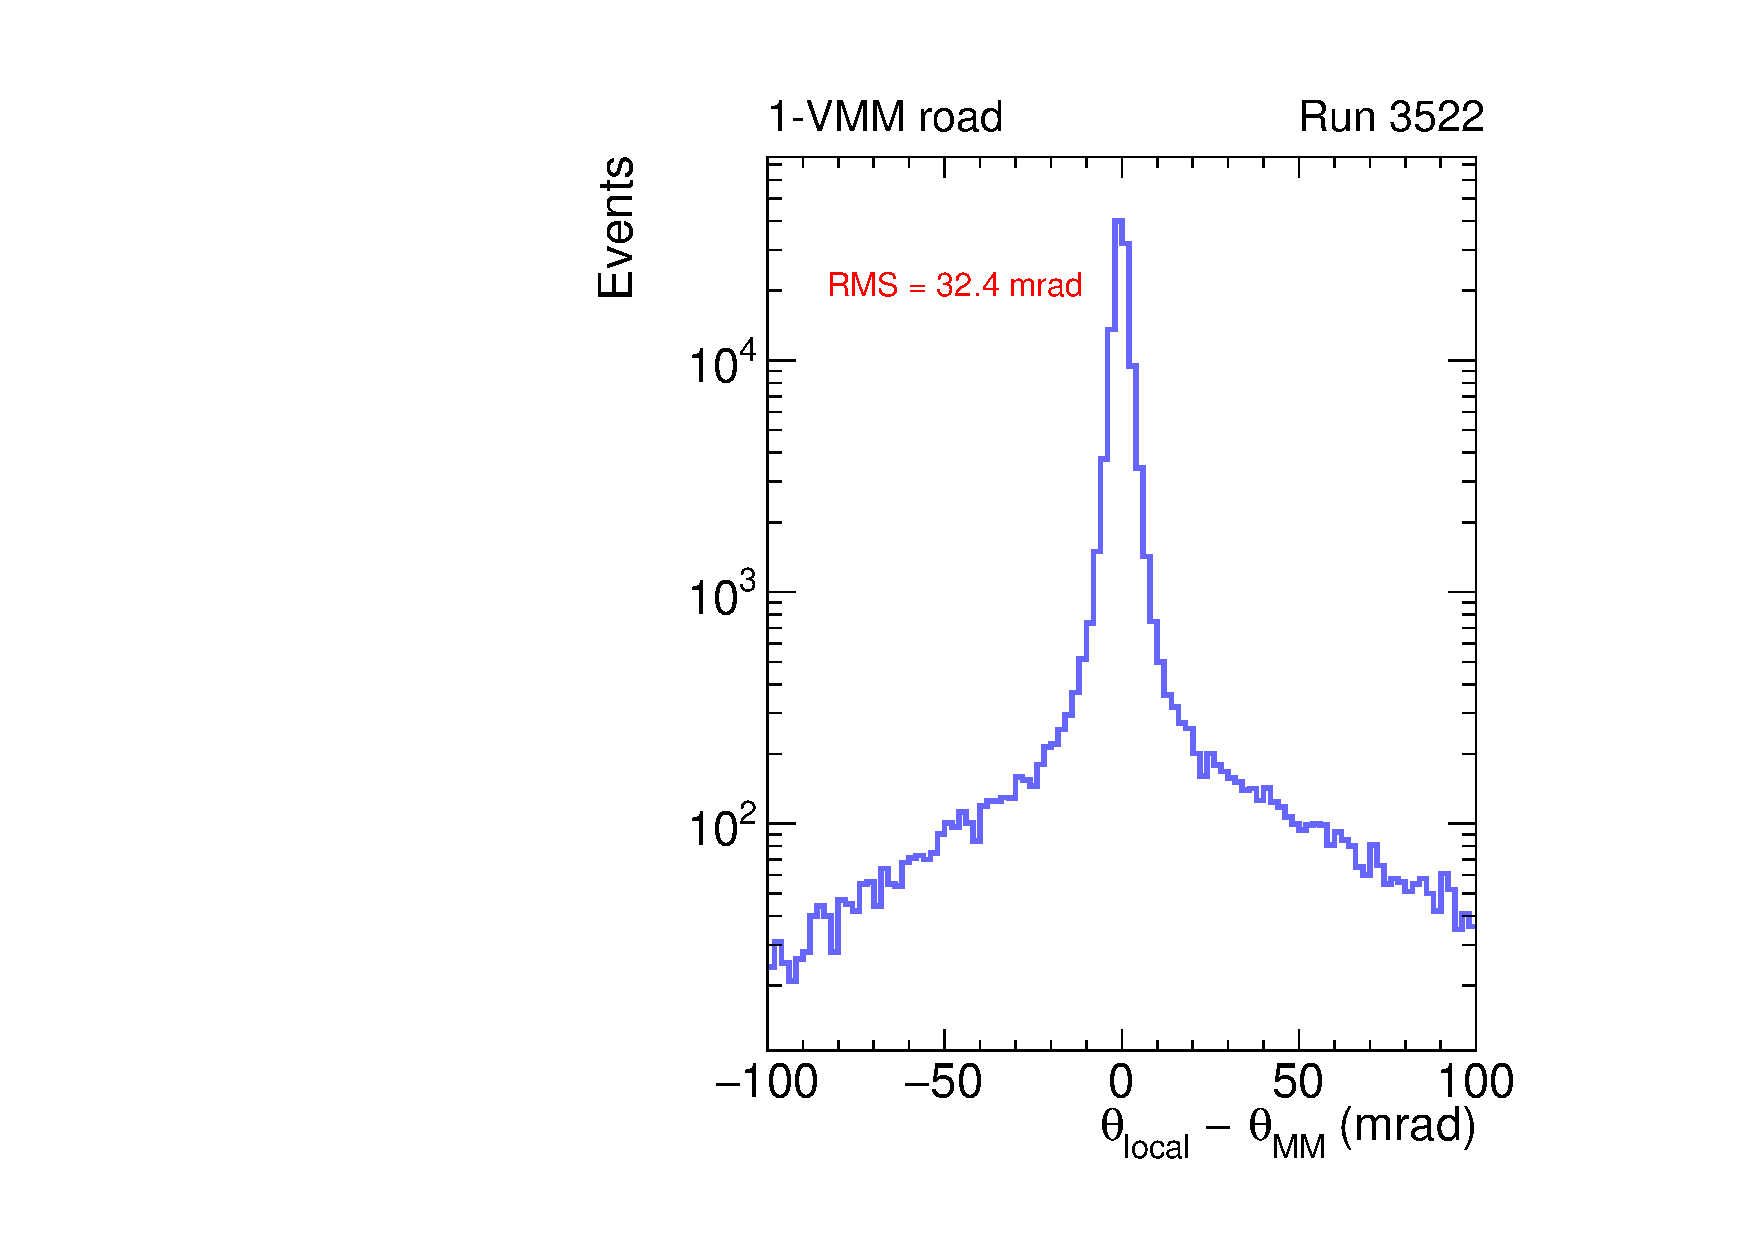
\includegraphics[width=0.4\textwidth]{figures/gbtanalysis3522/TP_angres_full.pdf}
    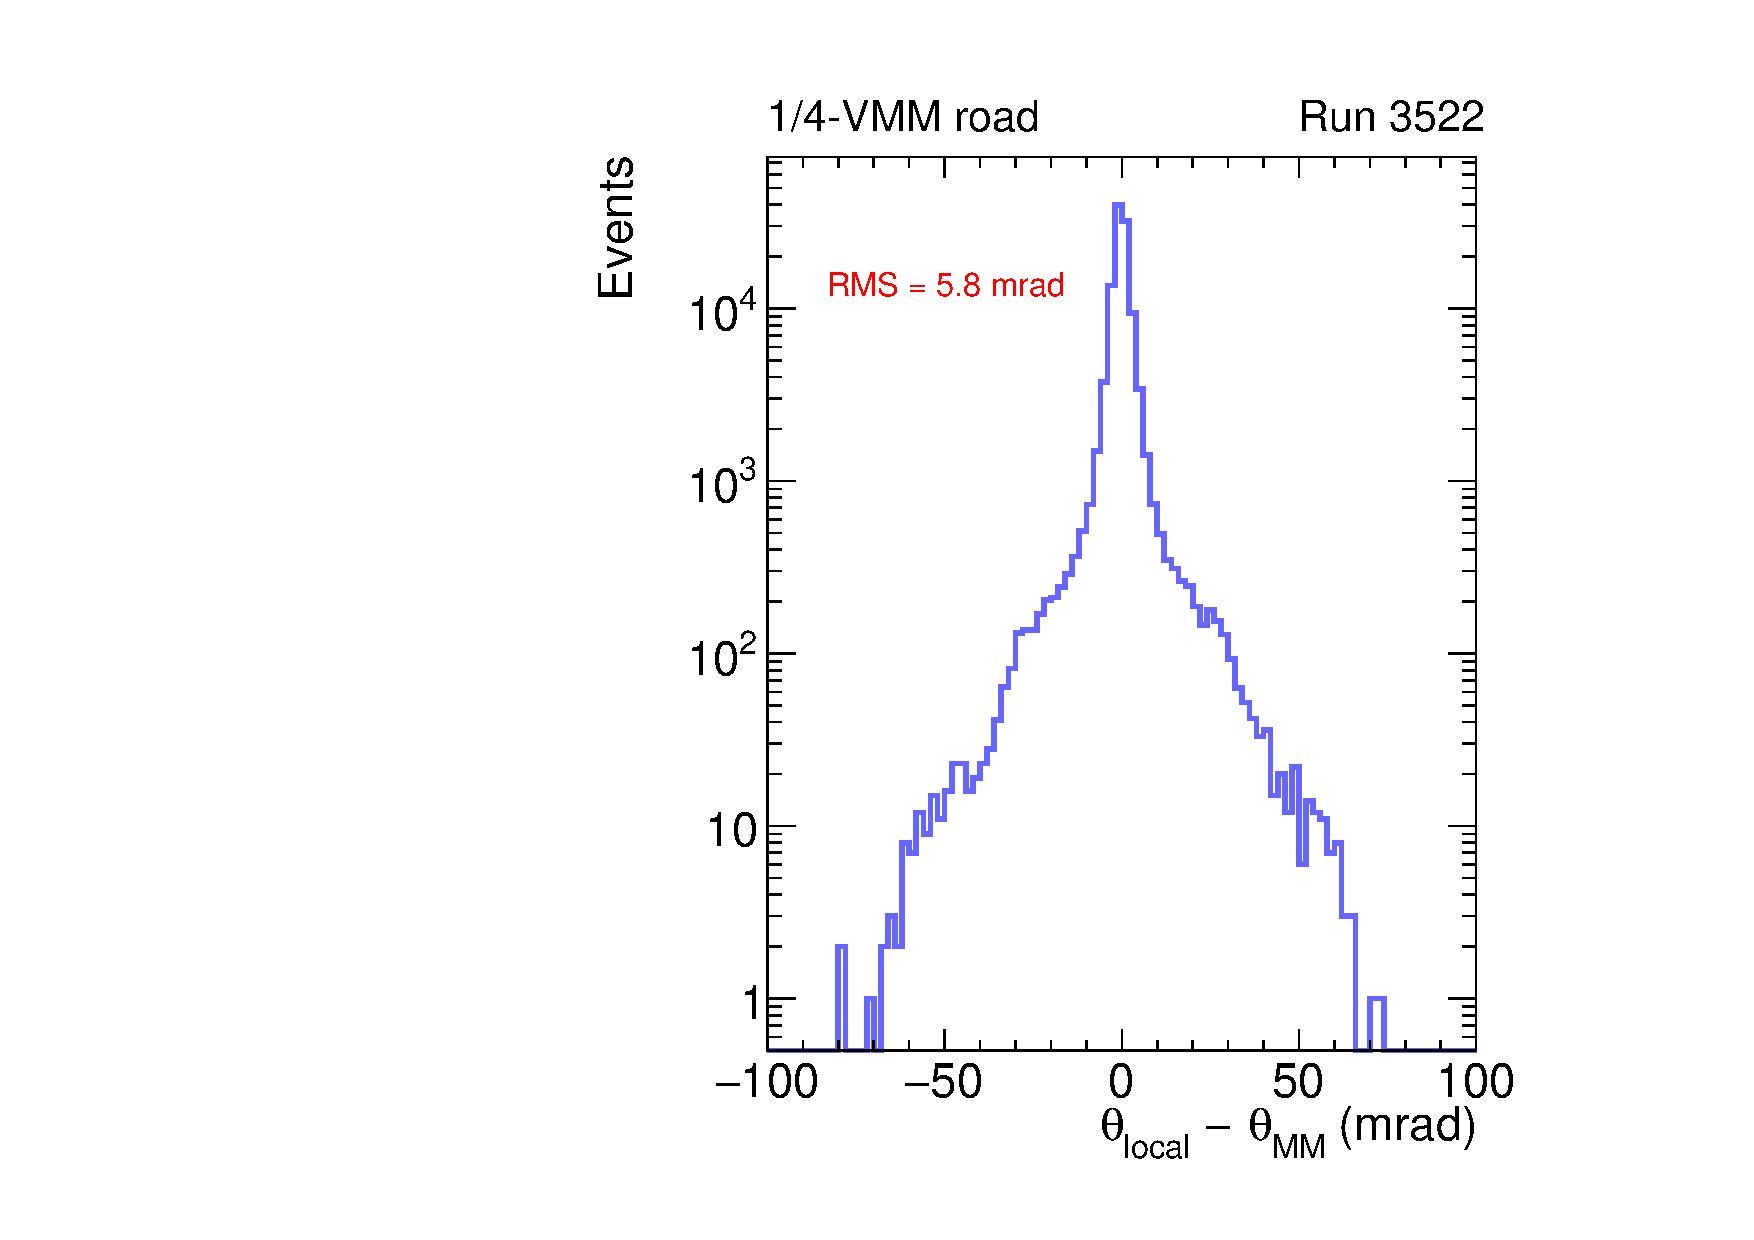
\includegraphics[width=0.4\textwidth]{figures/gbtanalysis3522/TP_angres.pdf}
  \end{center}
  \vspace{-10pt}
  \caption{The $\theta$ resolution of the MM TP relative to the full readout, using 1-VMM online roads (left) and 1/4-VMM offline roads (right). The tails of the resolution are greatly suppressed with smaller roads.}
  \label{fig:thetares}
\end{figure}


\subsubsection{Time resolution}

\begin{figure}[!htpb]
  \begin{center}
    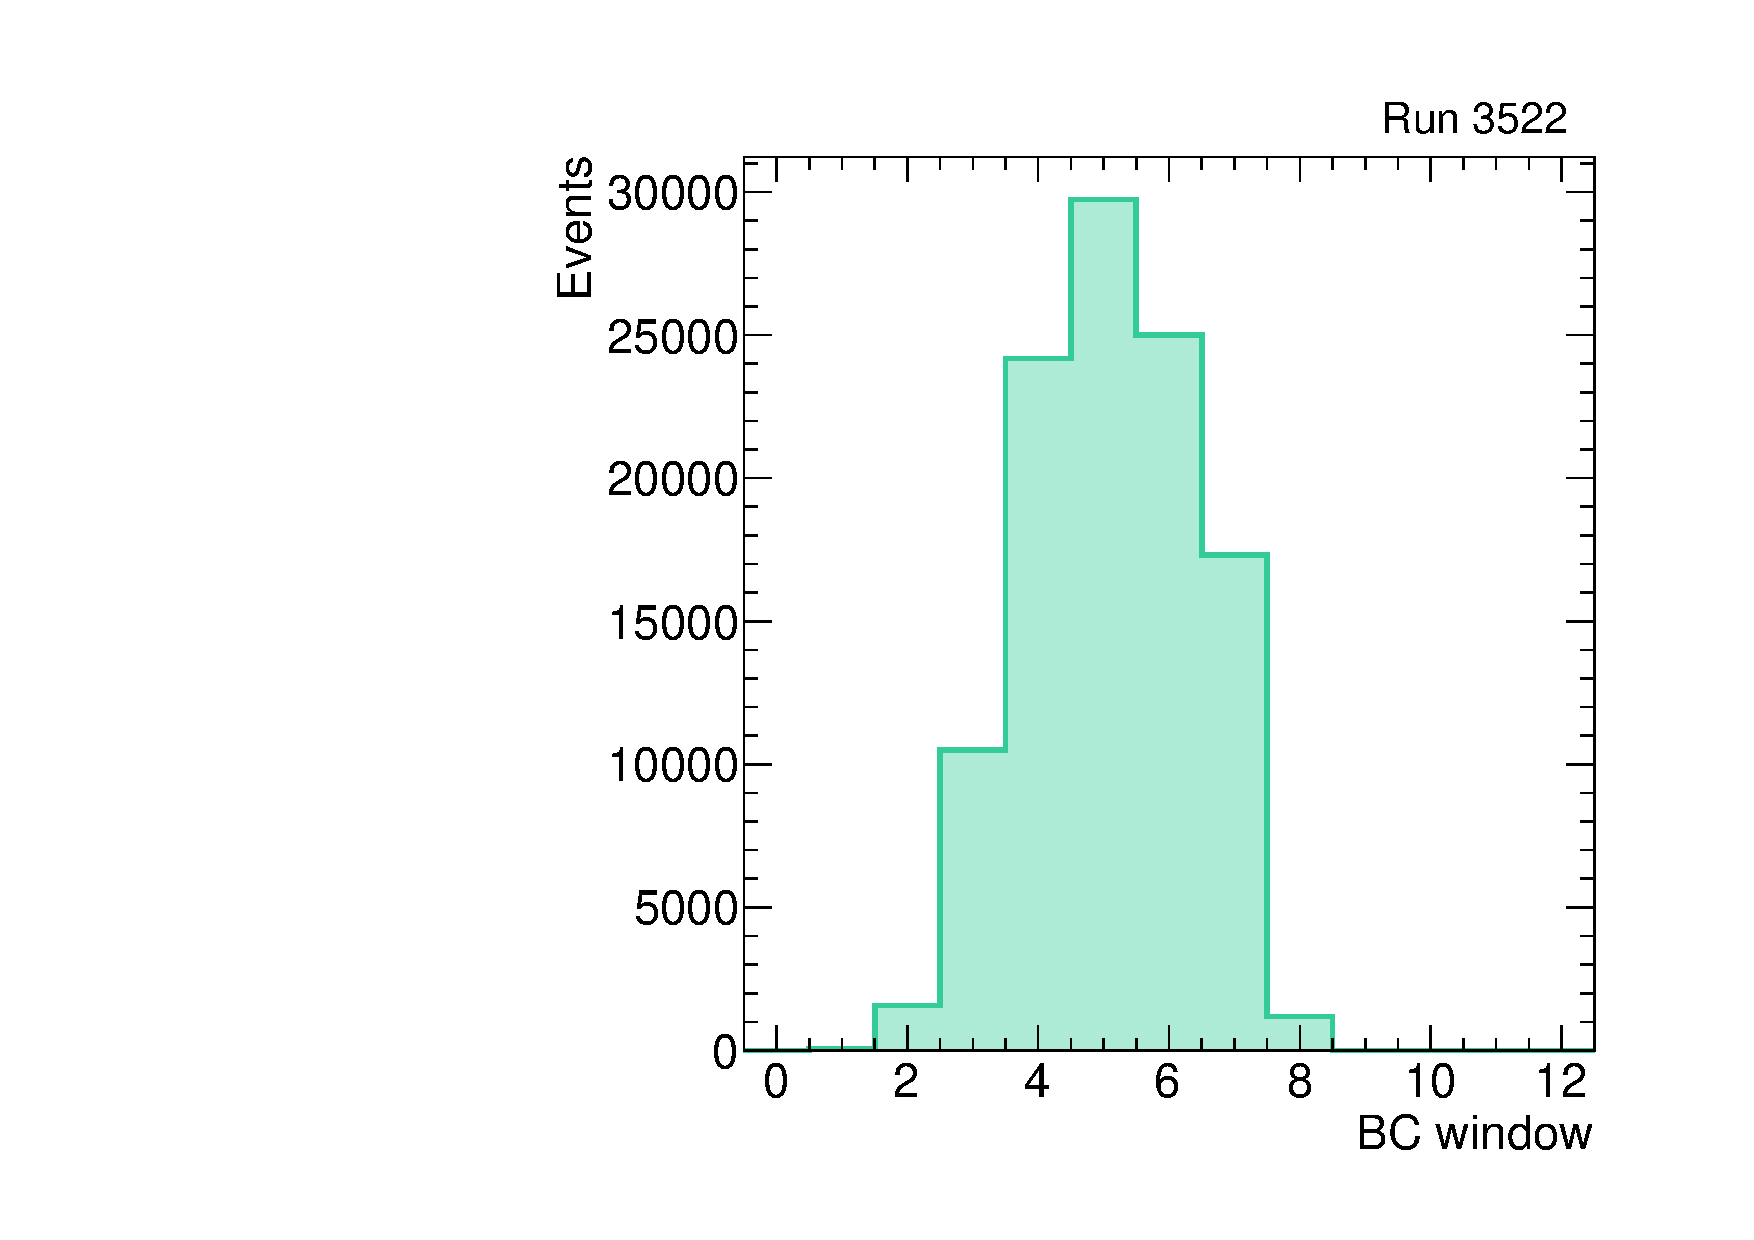
\includegraphics[width=0.4\textwidth]{figures/gbtanalysis3522/artwin_lin.pdf}
    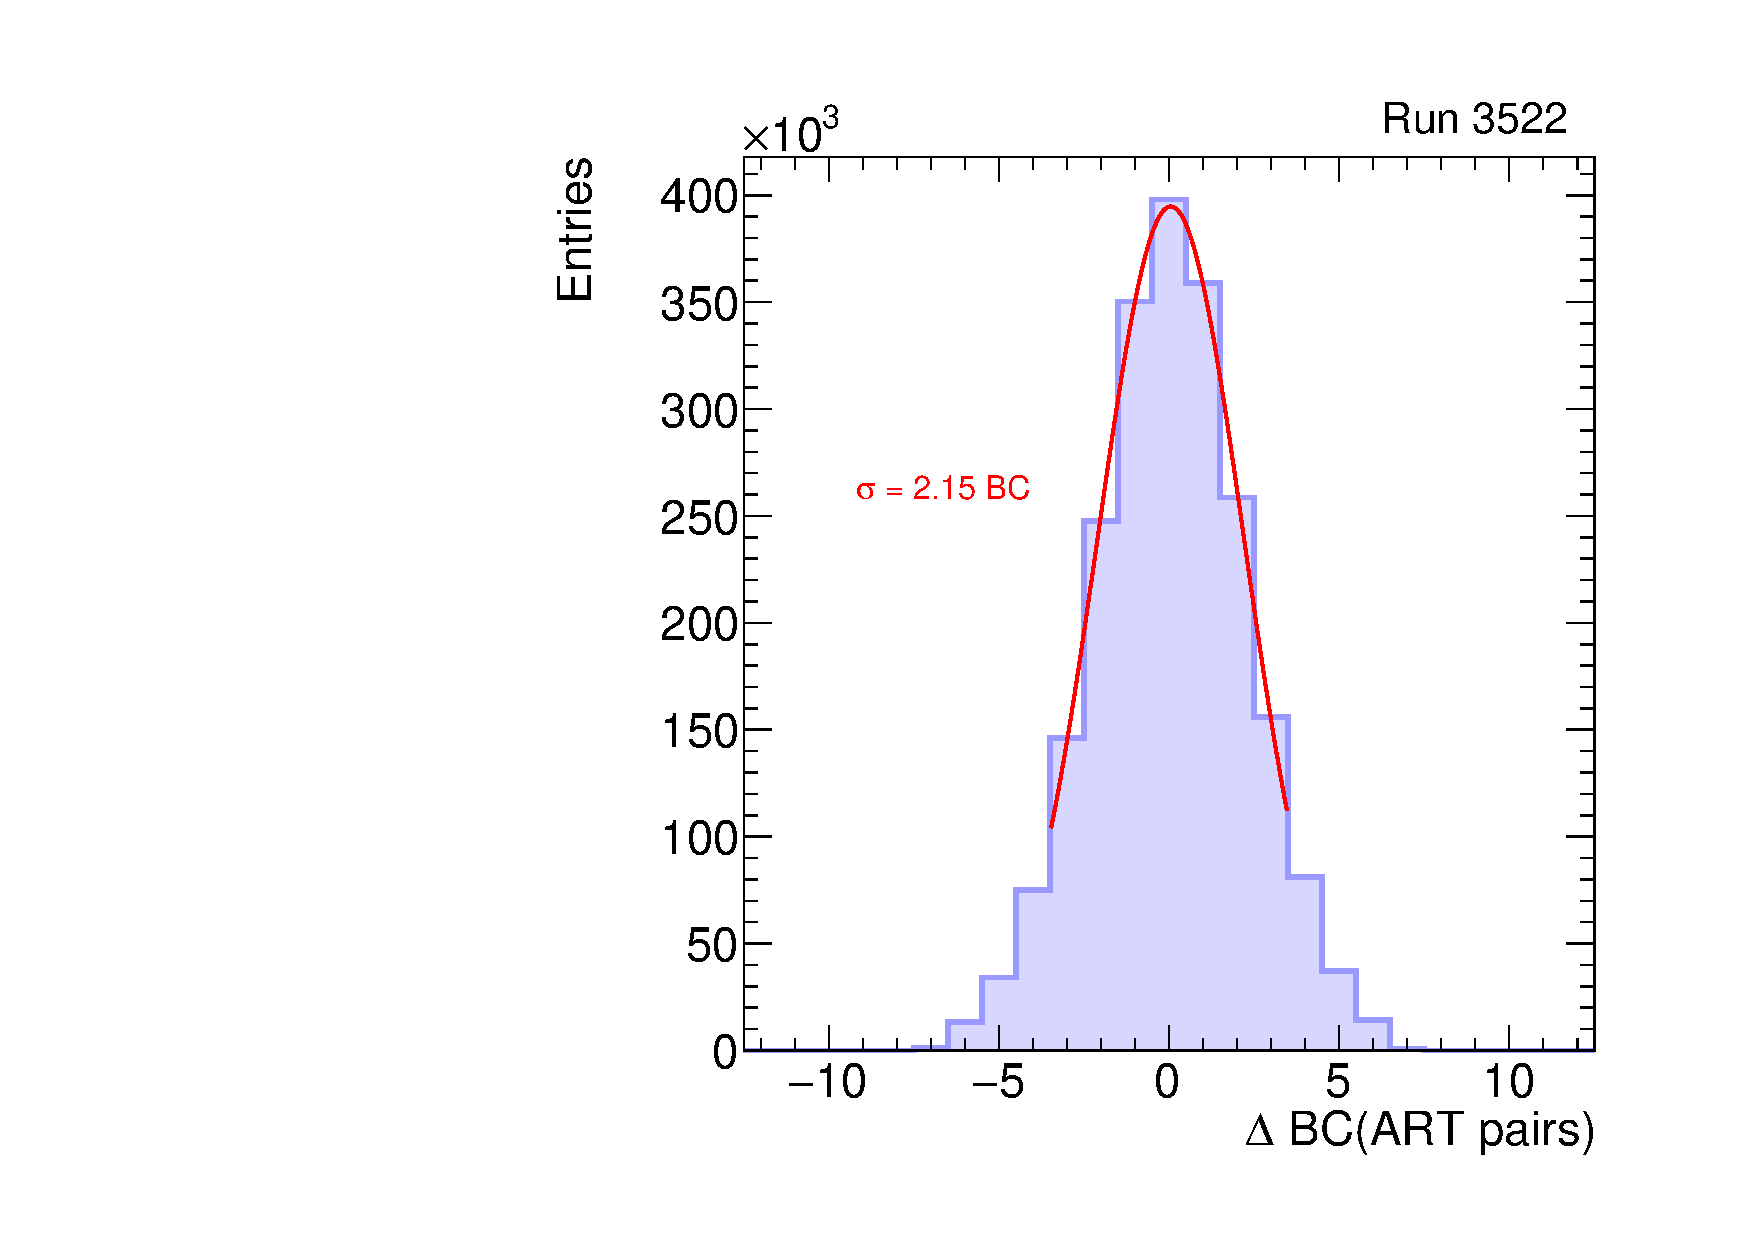
\includegraphics[width=0.4\textwidth]{figures/gbtanalysis3522/artrpairs_lin.pdf}
  \end{center}
  \vspace{-10pt}
  \caption{The time window required to record all hits in a trigger (left) and the $\Delta\text{BC}$ of all pairs of hits in a trigger (right). A gaussian fit is overlaid on the distribution of $\Delta\text{BC}$ and describes the data well.}
  \label{fig:time}
\end{figure}

\begin{figure}[!htpb]
  \begin{center}
    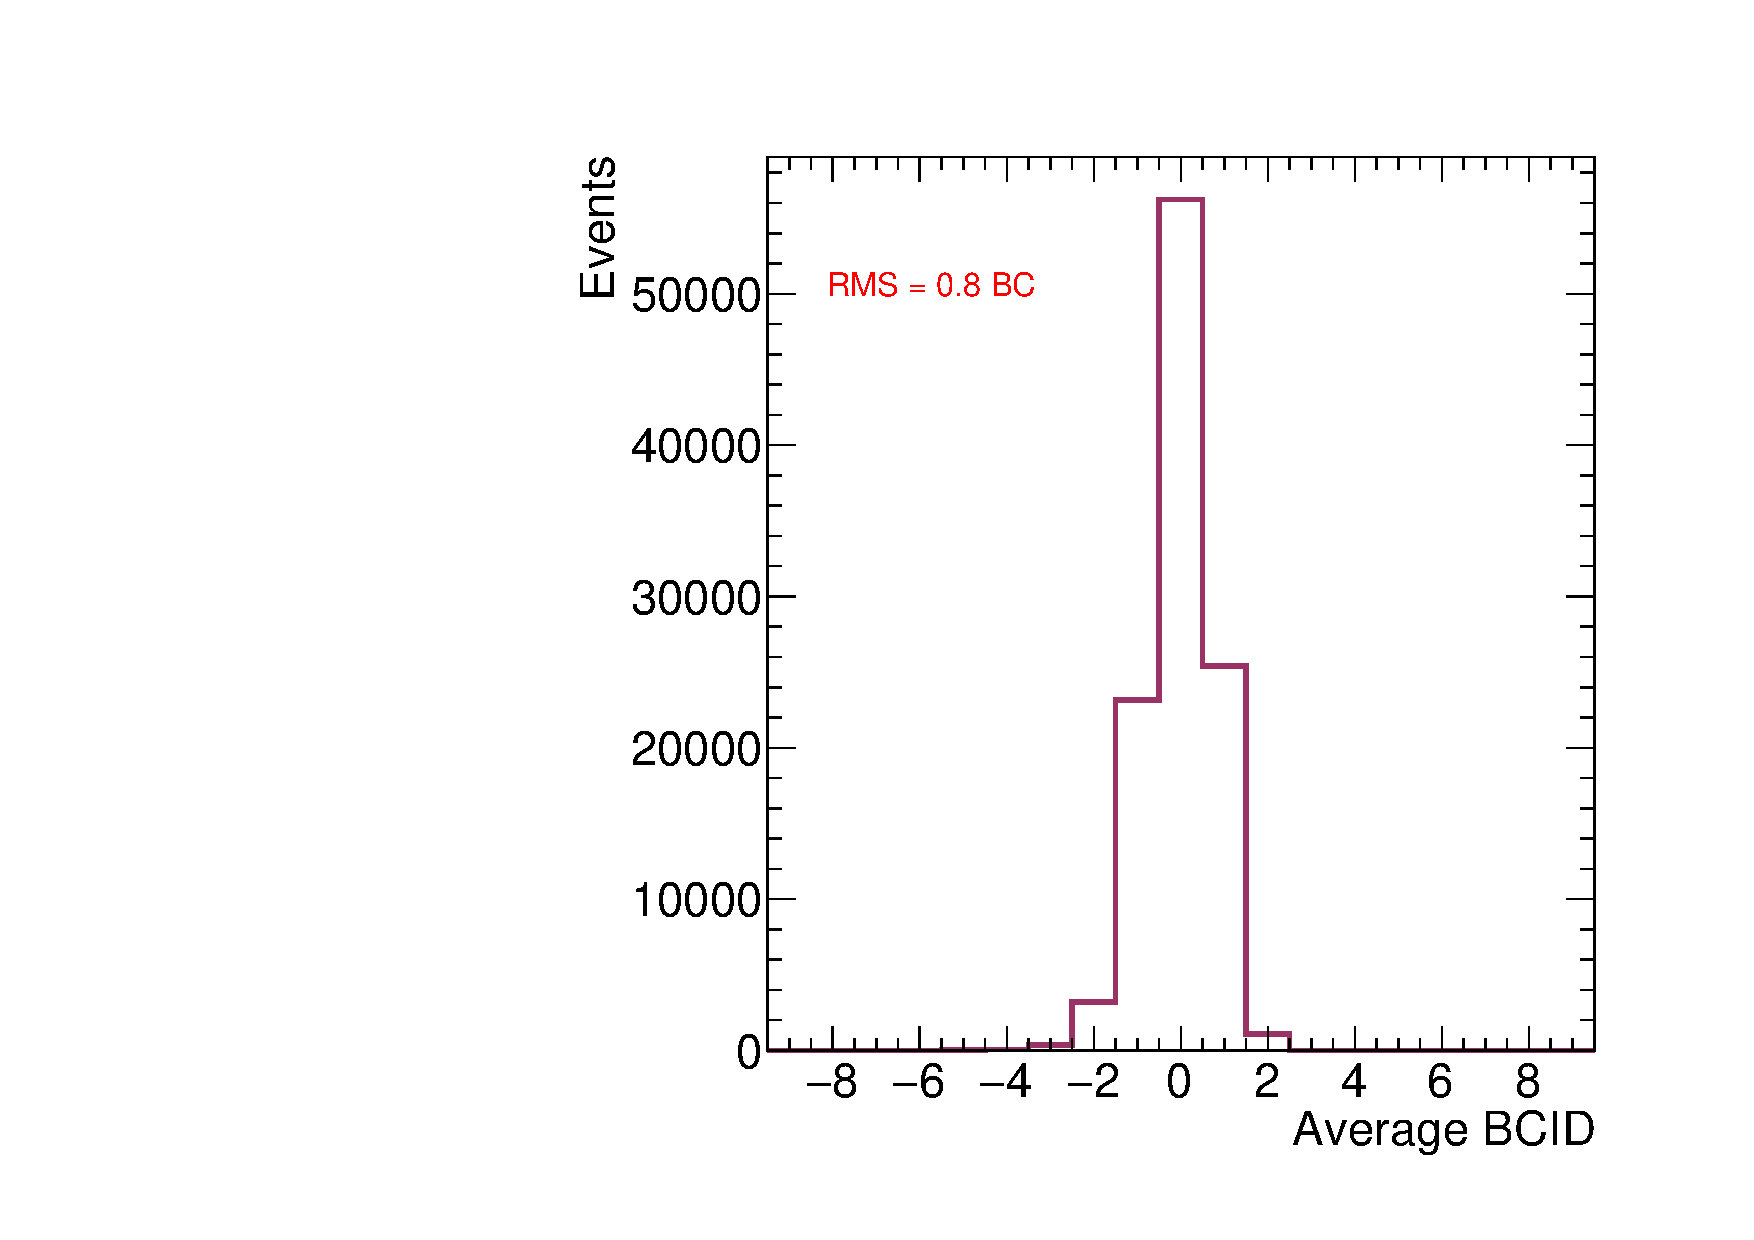
\includegraphics[width=0.4\textwidth]{figures/gbtanalysis3522/avg_BCID.pdf}
    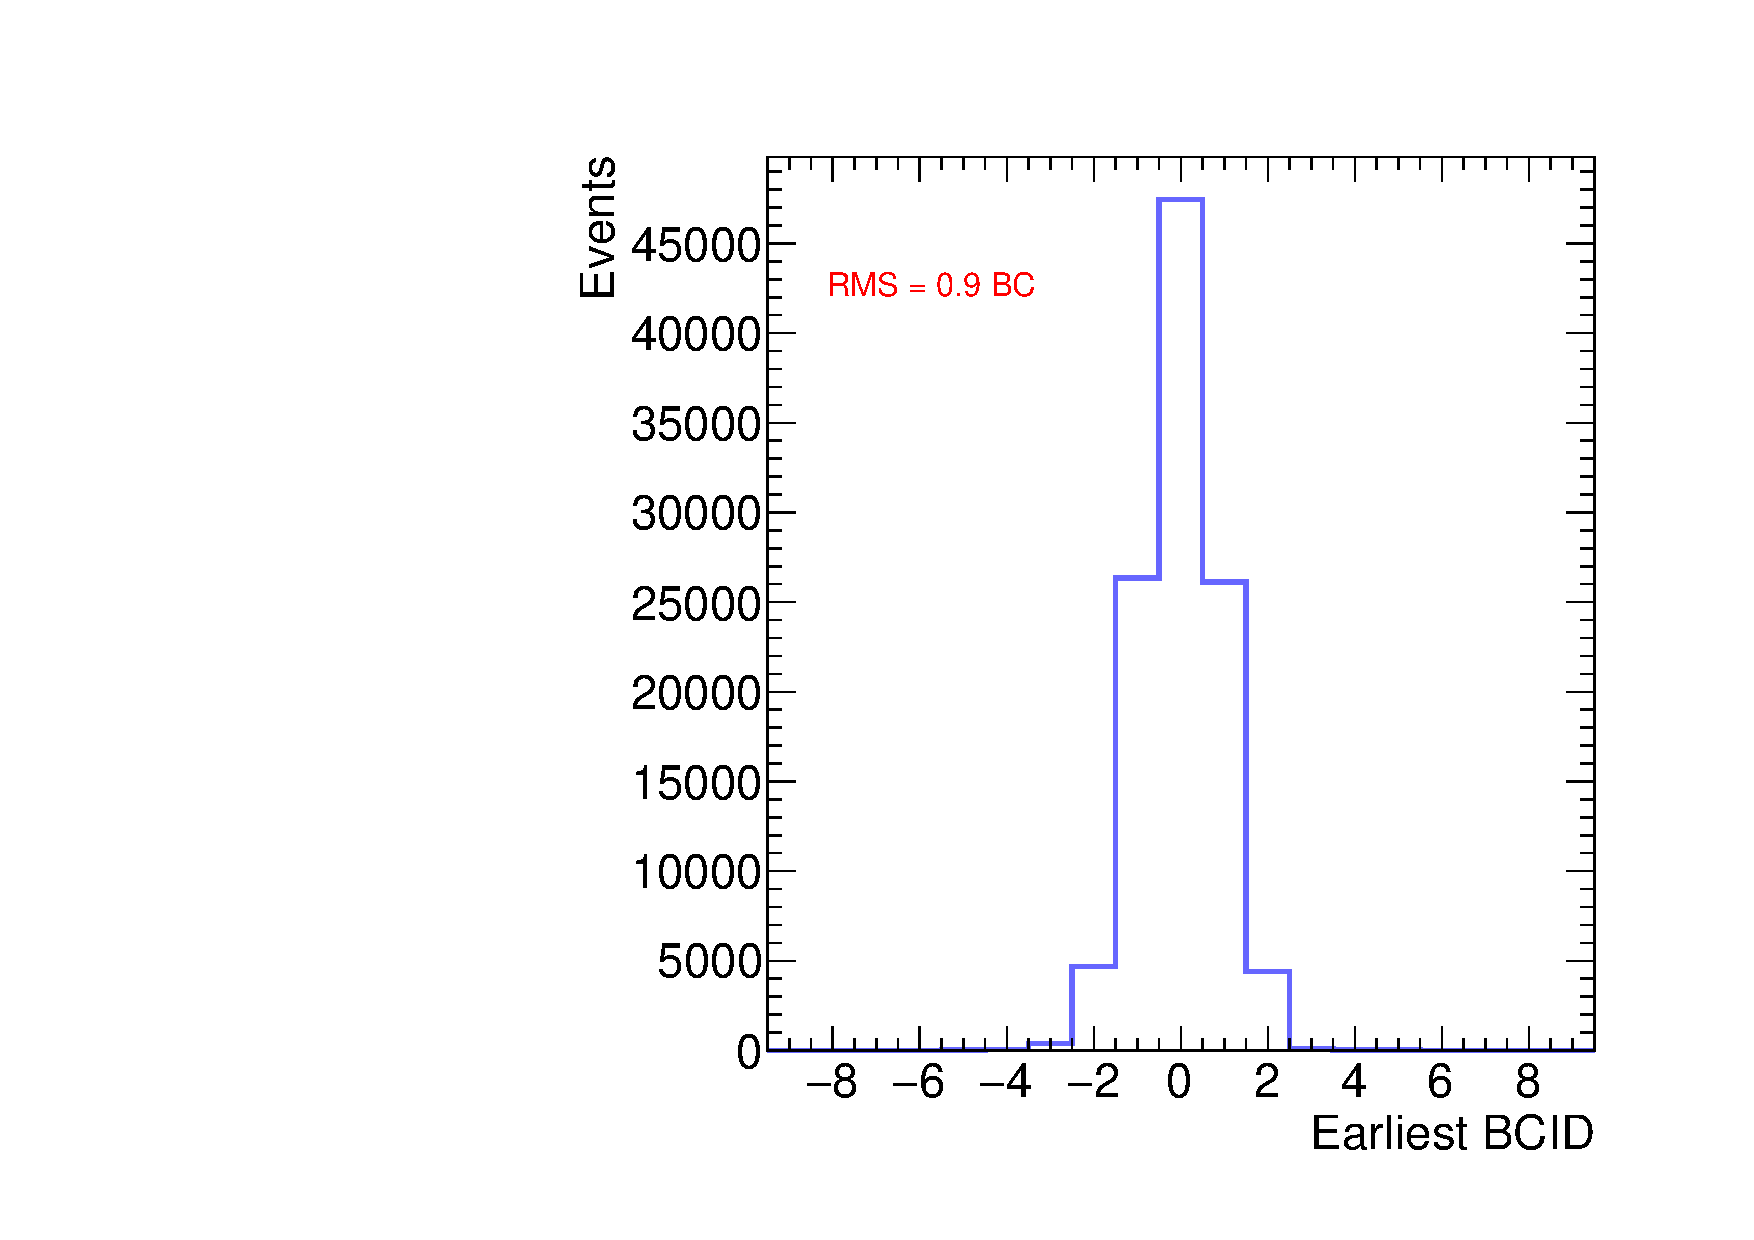
\includegraphics[width=0.4\textwidth]{figures/gbtanalysis3522/earliest_BCID.pdf}
  \end{center}
  \vspace{-10pt}
  \caption{The time resolution of the MM TP relative to the scintillator. The BCID of the trigger can be defined as the average BCID of the ART hits (left) or the earliest BCID (right). Choosing the average BCID has better resolution than choosing the earliest.}
  \label{fig:timeres}
\end{figure}

\subsection{Integration time}
\label{sec:perf-integ}

